\documentclass{article}
\usepackage{graphicx}
\usepackage[utf8]{inputenc}
\usepackage[a4paper, total={6in, 8in}]{geometry}
\usepackage{fancyhdr}
\usepackage{subcaption}
\usepackage{xcolor}
\usepackage[hidelinks]{hyperref}

\pagestyle{fancy}
\fancyhf{}
\fancyfoot[L]{Alessandro Dori}
\fancyfoot[R]{\thepage}
\fancyhead[L]{Interazione Uomo Macchina}
\fancyhead[R]{SmartCycle}
\renewcommand{\headrulewidth}{0.4pt}
\renewcommand{\footrulewidth}{0.4pt}

\begin{document}
\begin{center}
    \Huge Progetto Interazione Uomo Macchina
        \vspace{0.5cm}

        \large A.A. 2024/2025 - Alessandro Dori 1843237
        \vspace{1cm}

        \large \textsf{\textbf{SmartCycle}}

        \includegraphics[width=0.3\textwidth, trim=110 110 110 110, clip]{img/SM.png}
\end{center}

\tableofcontents
\newpage

\section{Introduzione}
L'obiettivo di questo documento è raccogliere le domande utilizzate durante le interviste per il progetto SmartCycle e gli appunti presi durante tali interviste.
Questo documento servirà come riferimento per le fasi successive del progetto, fornendo un'analisi delle risposte raccolte.

\section{Domande delle Interviste}
\begin{enumerate}
    \item Nome?
    \item Età?
    \item Con chi vivi?
    \item Città di residenza?
    \item Quanto tempo dedichi alla preparazione dei pasti durante la settimana?
    \item Quanto tempo dedichi alla spesa alimentare durante la settimana?
    \item Quali difficoltà incontri nella gestione degli sprechi alimentari?
    \item Utilizzi già qualche sistema o applicazione per ridurre gli sprechi alimentari? Se si, quale? (Se non si utilizza alcun sistema, saltare alla sezione Domande per utenti che non utilizzano applicazioni per acquistare cibo invenduto)
    \item Quando è stata l'ultima volta che hai utilizzato un'applicazione per acquistare cibo invenduto?
    \item Quanto spesso ti capita di acquistare cibo invenduto tramite applicazioni o altri sistemi?
    \item L'ultima volta che hai utilizzato un'applicazione per acquistare cibo invenduto, hai riscontrato qualche problema? Se si, quali?
    \item In base a cosa decidi di utilizzare un'applicazione per acquistare cibo invenduto rispetto ad andare direttamente di persona?
    \item Quali sono i fattori che ti spingono a scegliere una pizzeria/hamburgeria o un ristorante rispetto ad un altro quando utilizzi queste applicazioni?
\end{enumerate}

\paragraph{Domande per utenti che non utilizzano applicazioni per acquistare cibo invenduto}
\label{dom_non_utilizzatori}
\begin{enumerate}
    \item Se no, come mai non hai mai utilizzato un'applicazione per acquistare cibo invenduto?
    \item Cosa ti spingerebbe a utilizzare un'applicazione per acquistare cibo invenduto?
    \item Quali sarebbero le motivazioni per cui sceglieresti di utilizzare un applicazione per acquistare cibo invenduto (ipotizzando che la conosca) rispetto ad andare direttamete di persona?
    \item Cosa ti spingerebbe a scegliere una pizzeria/hamburgeria o un ristorante rispetto ad un altro ipotizzando che tu utilizzassi queste applicazioni?
\end{enumerate}

\section{Motivazione delle Domande}
Le domande sono state pensate per capire meglio le abitudini alimentari delle persone e le loro opinioni riguardo lo spreco alimentare, ma anche per capire quante persone al giorno d'oggi siano informate dell'esistenza di applicazioni come Too Good To Go e Olio.
In particolare sono state fatte domande riguardo la frequenza con cui si butta cibo, la frequenza con cui si ordina cibo a domicilio, la frequenza con cui si cucina, la frequenza con cui si fa la spesa, e la frequenza con cui si utilizzano applicazioni per acquistare cibo invenduto.
\begin{itemize}
    \item Le prime 4 domande servono come riscaldamento per l'intervista (warm-up).
    \item La domanda 5 serve per capire quanto tempo le persone dedicano alla preparazione dei pasti e alla spesa alimentare, così da capire se la persona in questione possa essere un ottimo candidato/a per l'applicazione.
    \item Anche la domanda 6 mi permette di capire se la persona in questione possa essere un ottimo candidato/a per l'applicazione, chiedendogli quanto tempo dedica alla spesa alimentare.
    \item Le domande 7 e 8 servono per capire quali sono le difficoltà che le persone incontrano nella gestione degli sprechi alimentari ed eventualmente se conoscono già qualche sistema o applicazione per ridurli.
    \item Da qui le domande successive differiscono in base alla risposta alla domanda 8.
    \item Se la persona in questione utilizza già un sistema o un'applicazione per ridurre gli sprechi alimentari, le domande successive procedono dallo stesso elenco.
    \begin{itemize}
        \item La domanda 9 serve per capire quanto tempo è passato dall'ultima volta che la persona in questione ha utilizzato un'applicazione per acquistare cibo invenduto.
        \item La domanda 10 serve per capire la frequenza con cui utilizza applicazioni per acquistare cibo invenduto. (nel caso di "bugie" verrà smentito dalle domande precedenti)
        \item La domanda 11 serve per capire quali sono i motivi che spingono la persona in questione a utilizzare un'applicazione (i vantaggi).
    \end{itemize}
    \item Se la persona in questione non utilizza alcun sistema o applicazione per ridurre gli sprechi alimentari, le domande successive procedono dall'\hyperref[dom_non_utilizzatori]{\textcolor{blue}{elenco}} delle domande per utenti che non utilizzano applicazioni per acquistare cibo invenduto.
    \begin{itemize}
        \item La domanda 1 del secondo elenco serve per capire perché la persona in questione non ha mai utilizzato un'applicazione per acquistare cibo invenduto.
        \item La domanda 2 del secondo elenco serve per capire cosa spingerebbe la persona in questione a utilizzare un'applicazione per acquistare cibo invenduto.
        \item La domanda 3 del secondo elenco serve per capire quali sarebbero le motivazioni per cui la persona in questione sceglierebbe di utilizzare un'applicazione, ipotizzando che la conosca, per acquistare cibo invenduto rispetto ad andare direttamente di persona.
        \item La domanda 4 del secondo elenco serve per capire cosa spingerebbe la persona in questione a scegliere locale rispetto ad un altro ipotizzando che utilizzasse queste applicazioni.
    \end{itemize}
\end{itemize}

\newpage
\section{Appunti Presi}

\begin{figure}[h]
    \centering
    \begin{subfigure}{0.40\textwidth}
        \centering
        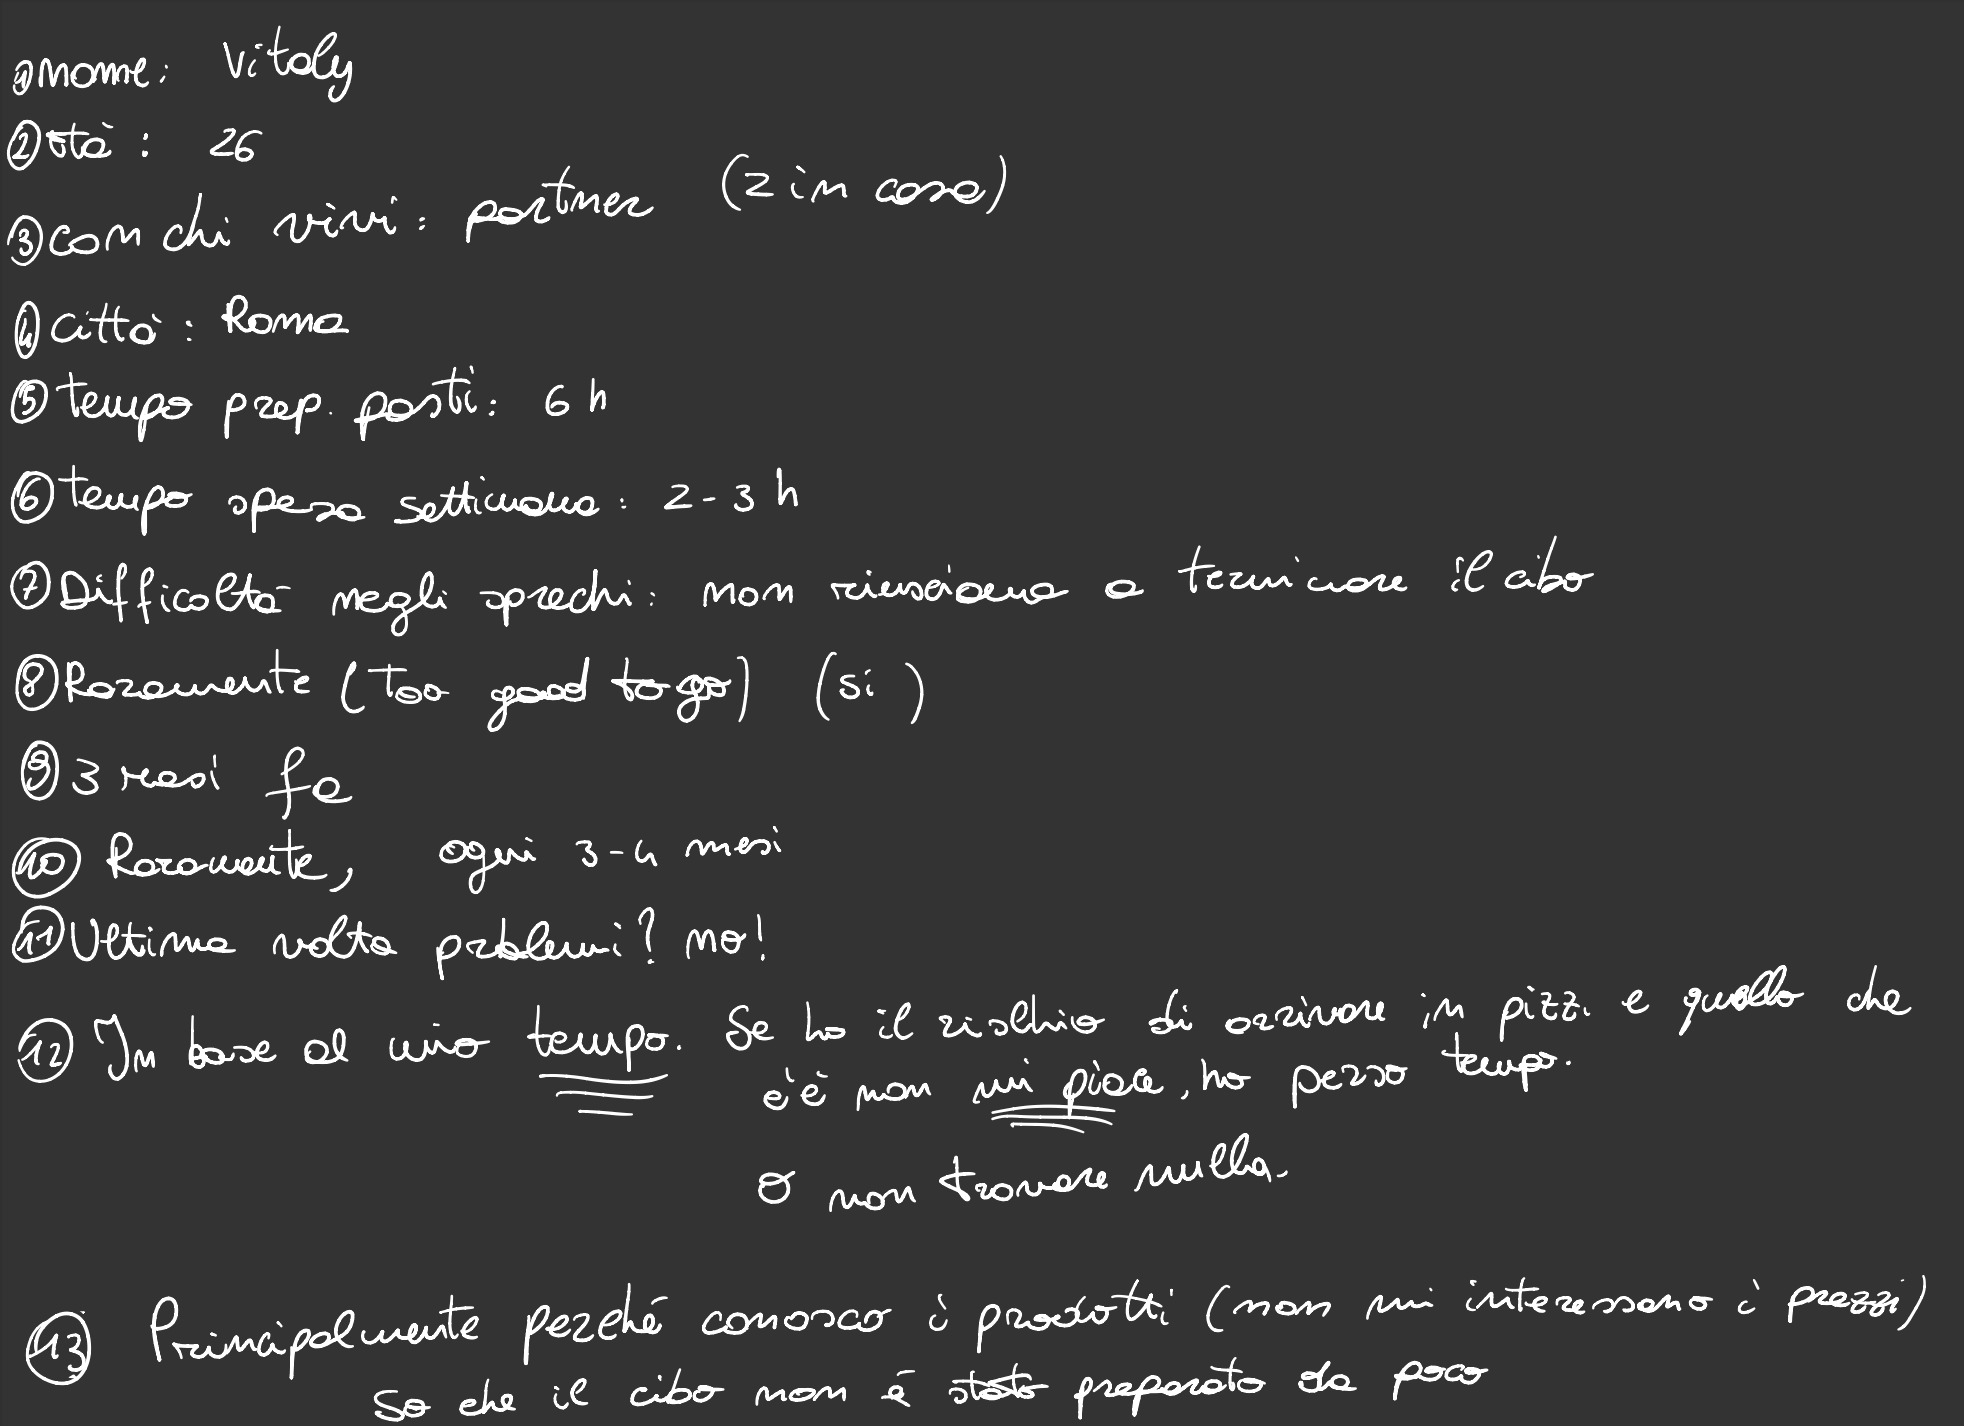
\includegraphics[width=\textwidth]{img/int1.png}
        \caption{Intervista 1}
    \end{subfigure}
    \hfill
    \begin{subfigure}{0.40\textwidth}
        \centering
        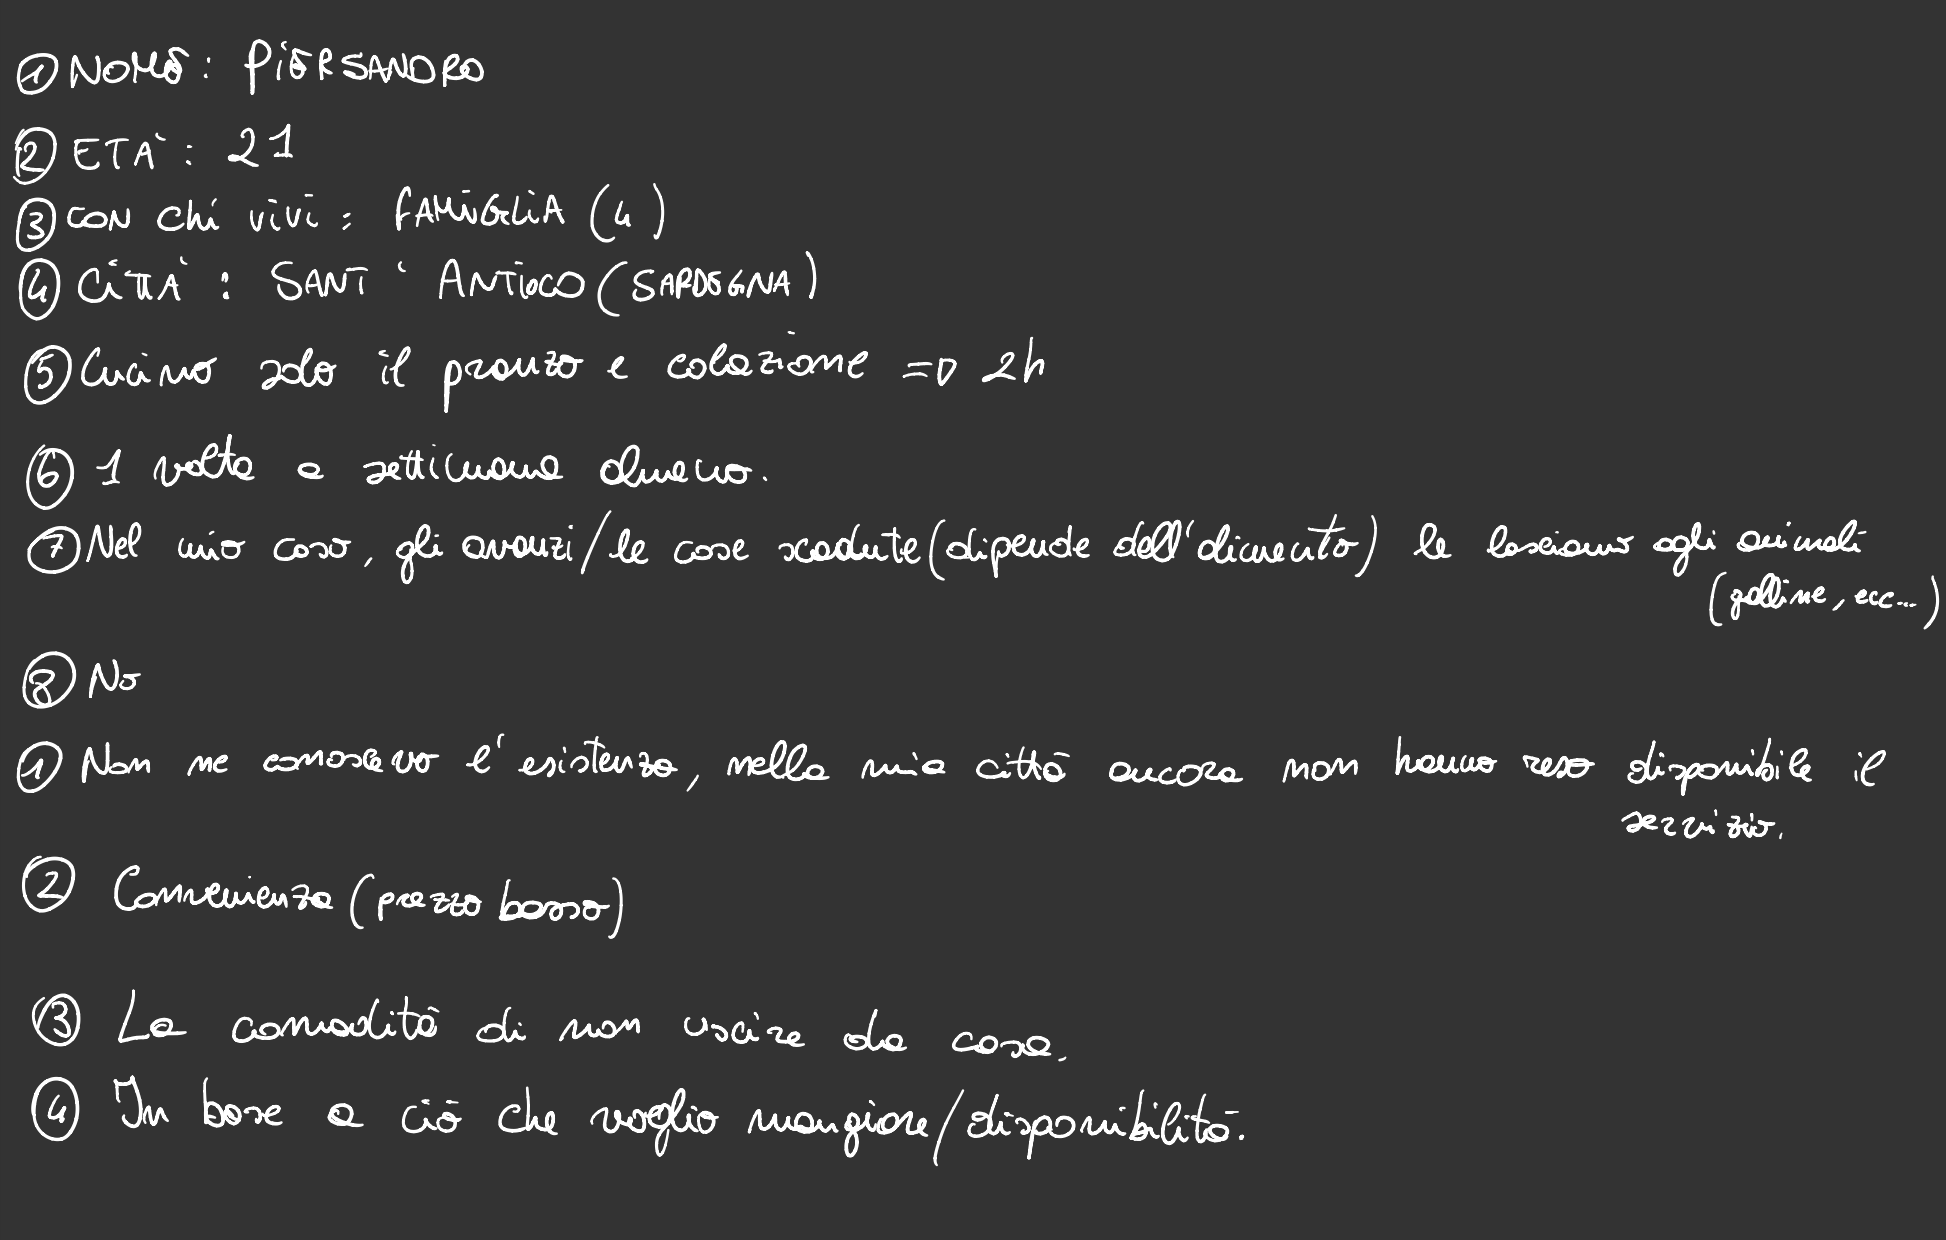
\includegraphics[width=\textwidth]{img/int2.png}
        \caption{Intervista 2}
    \end{subfigure}
\end{figure}

\begin{figure}[h]
    \centering
    \begin{subfigure}{0.40\textwidth}
        \centering
        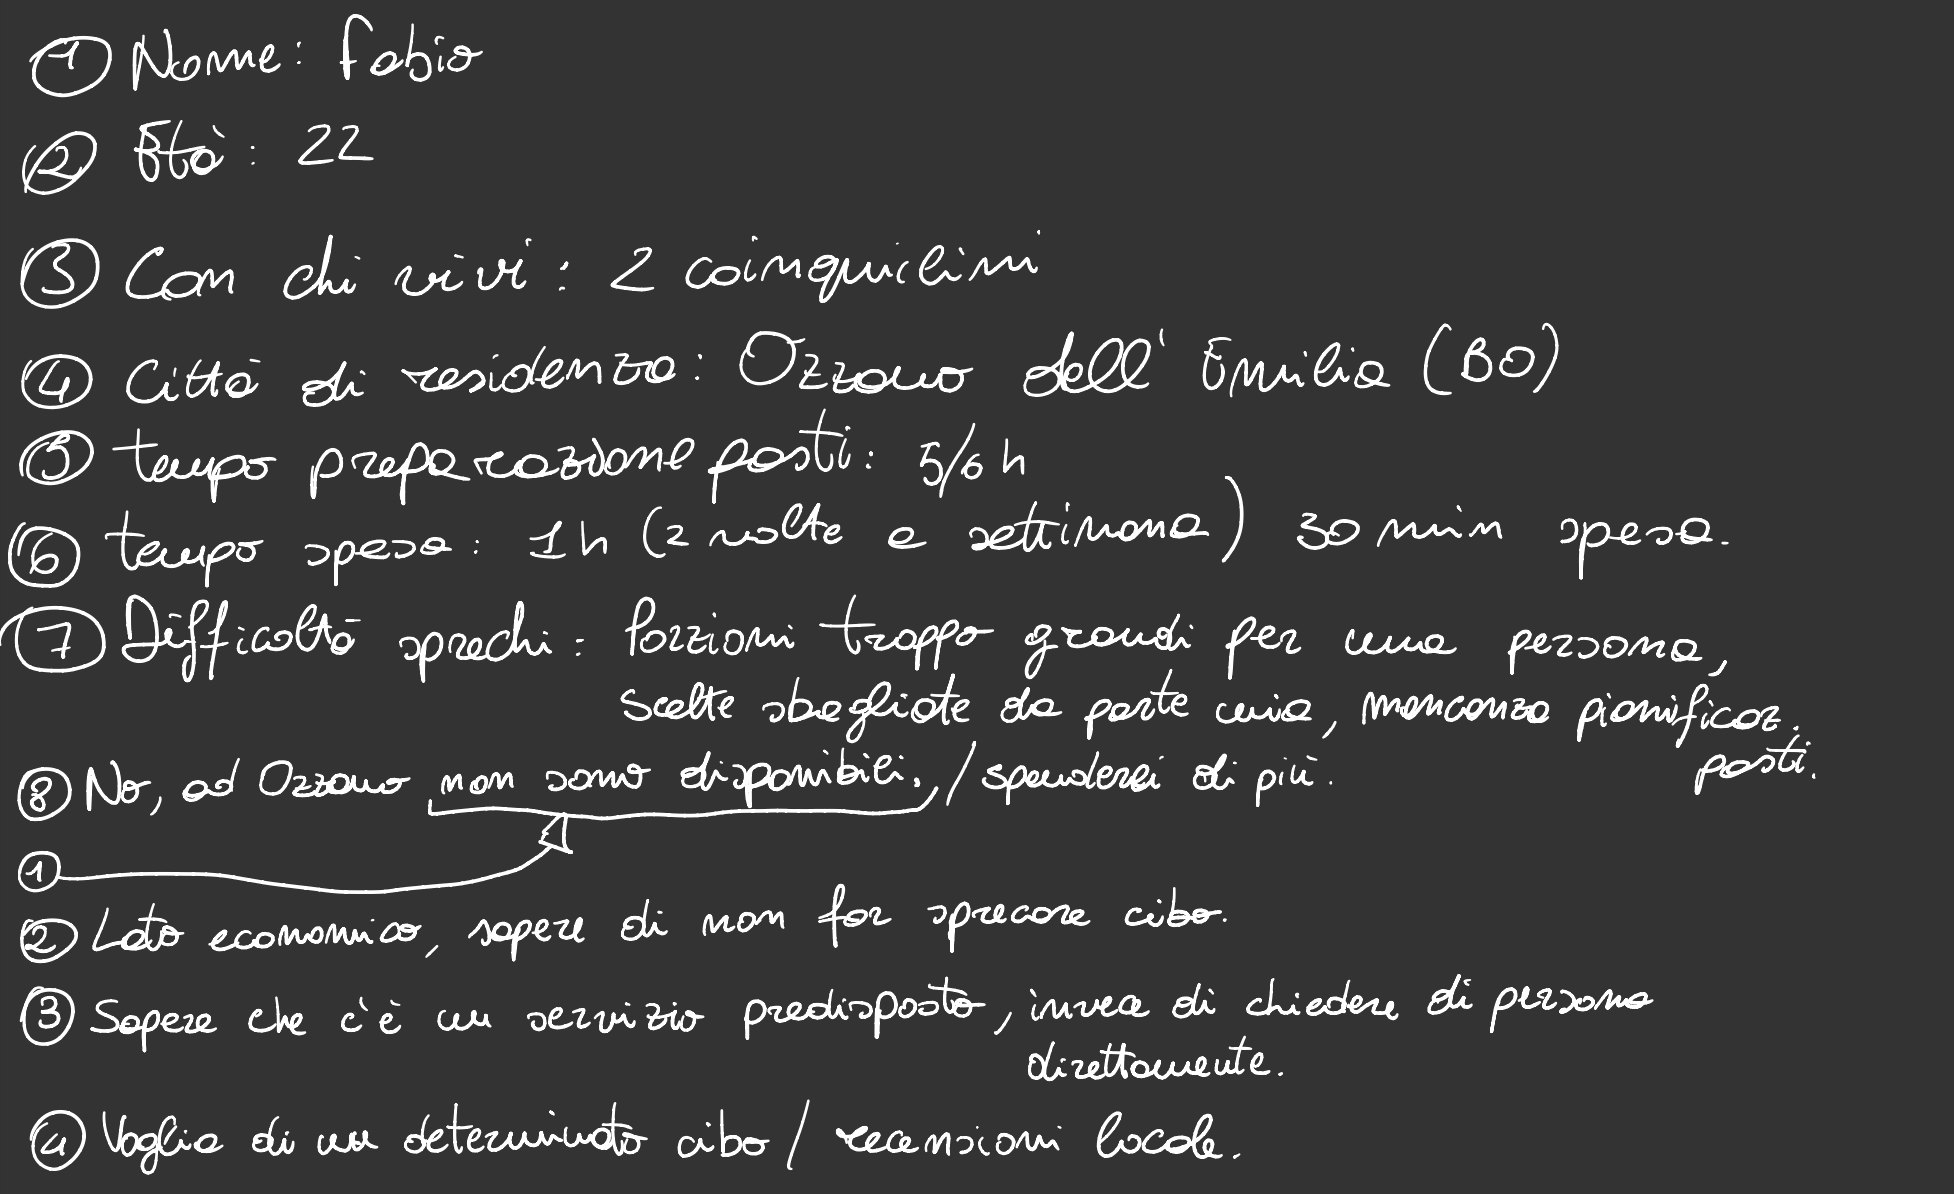
\includegraphics[width=\textwidth]{img/int3.png}
        \caption{Intervista 3}
    \end{subfigure}
    \hfill
    \begin{subfigure}{0.40\textwidth}
        \centering
        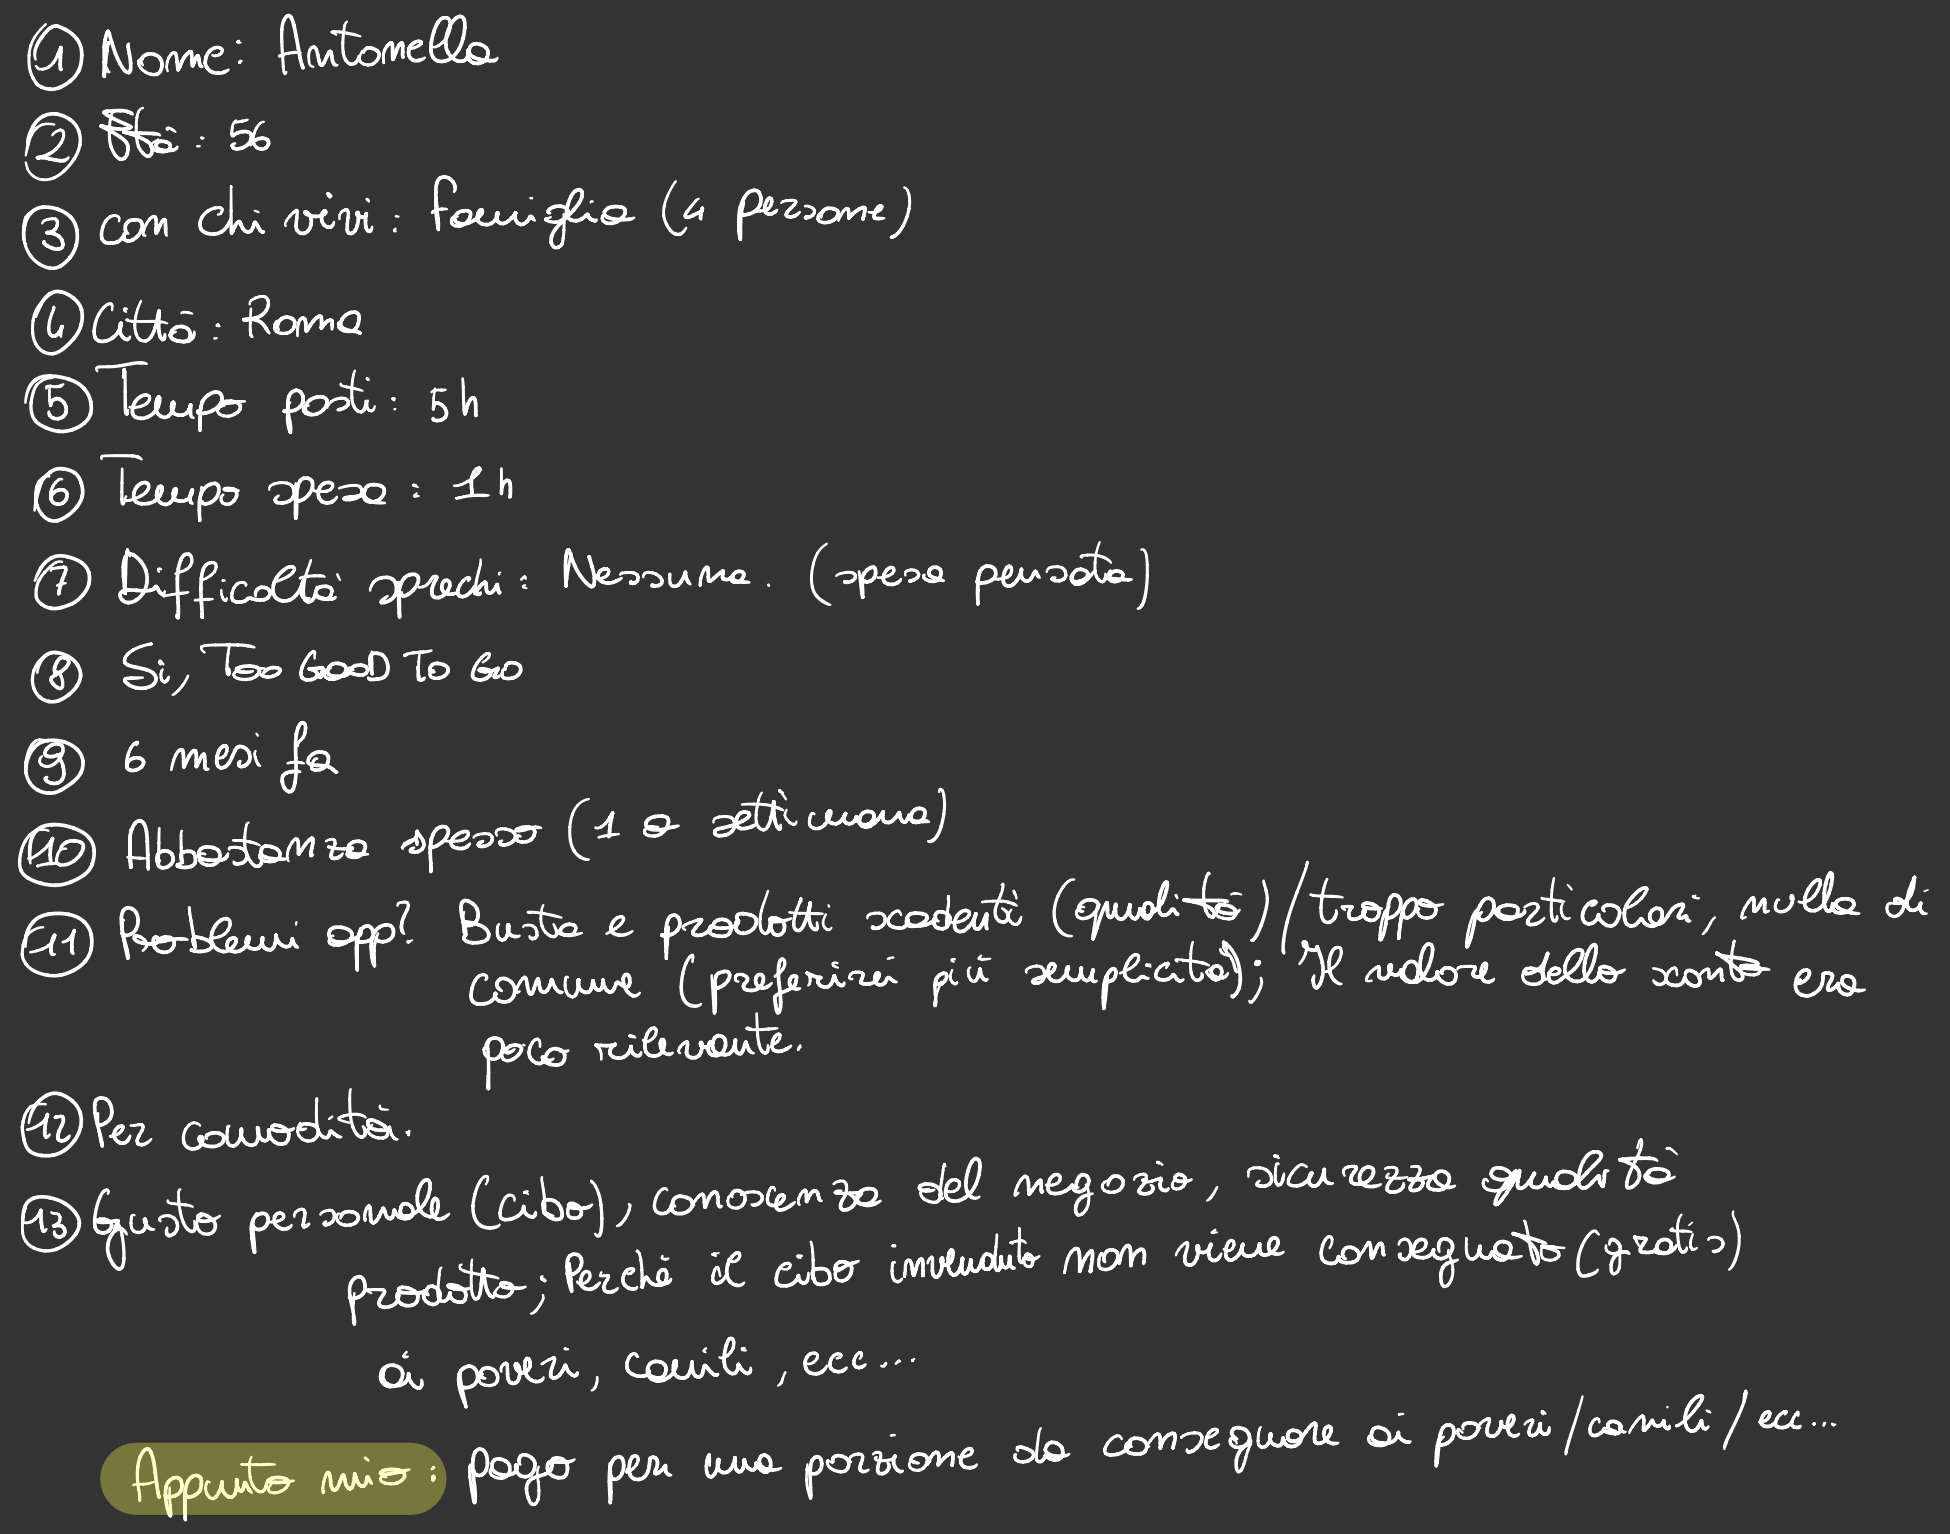
\includegraphics[width=\textwidth]{img/int4.png}
        \caption{Intervista 4}
    \end{subfigure}
\end{figure}

\begin{figure}[h]
    \centering
    \begin{subfigure}{0.40\textwidth}
        \centering
        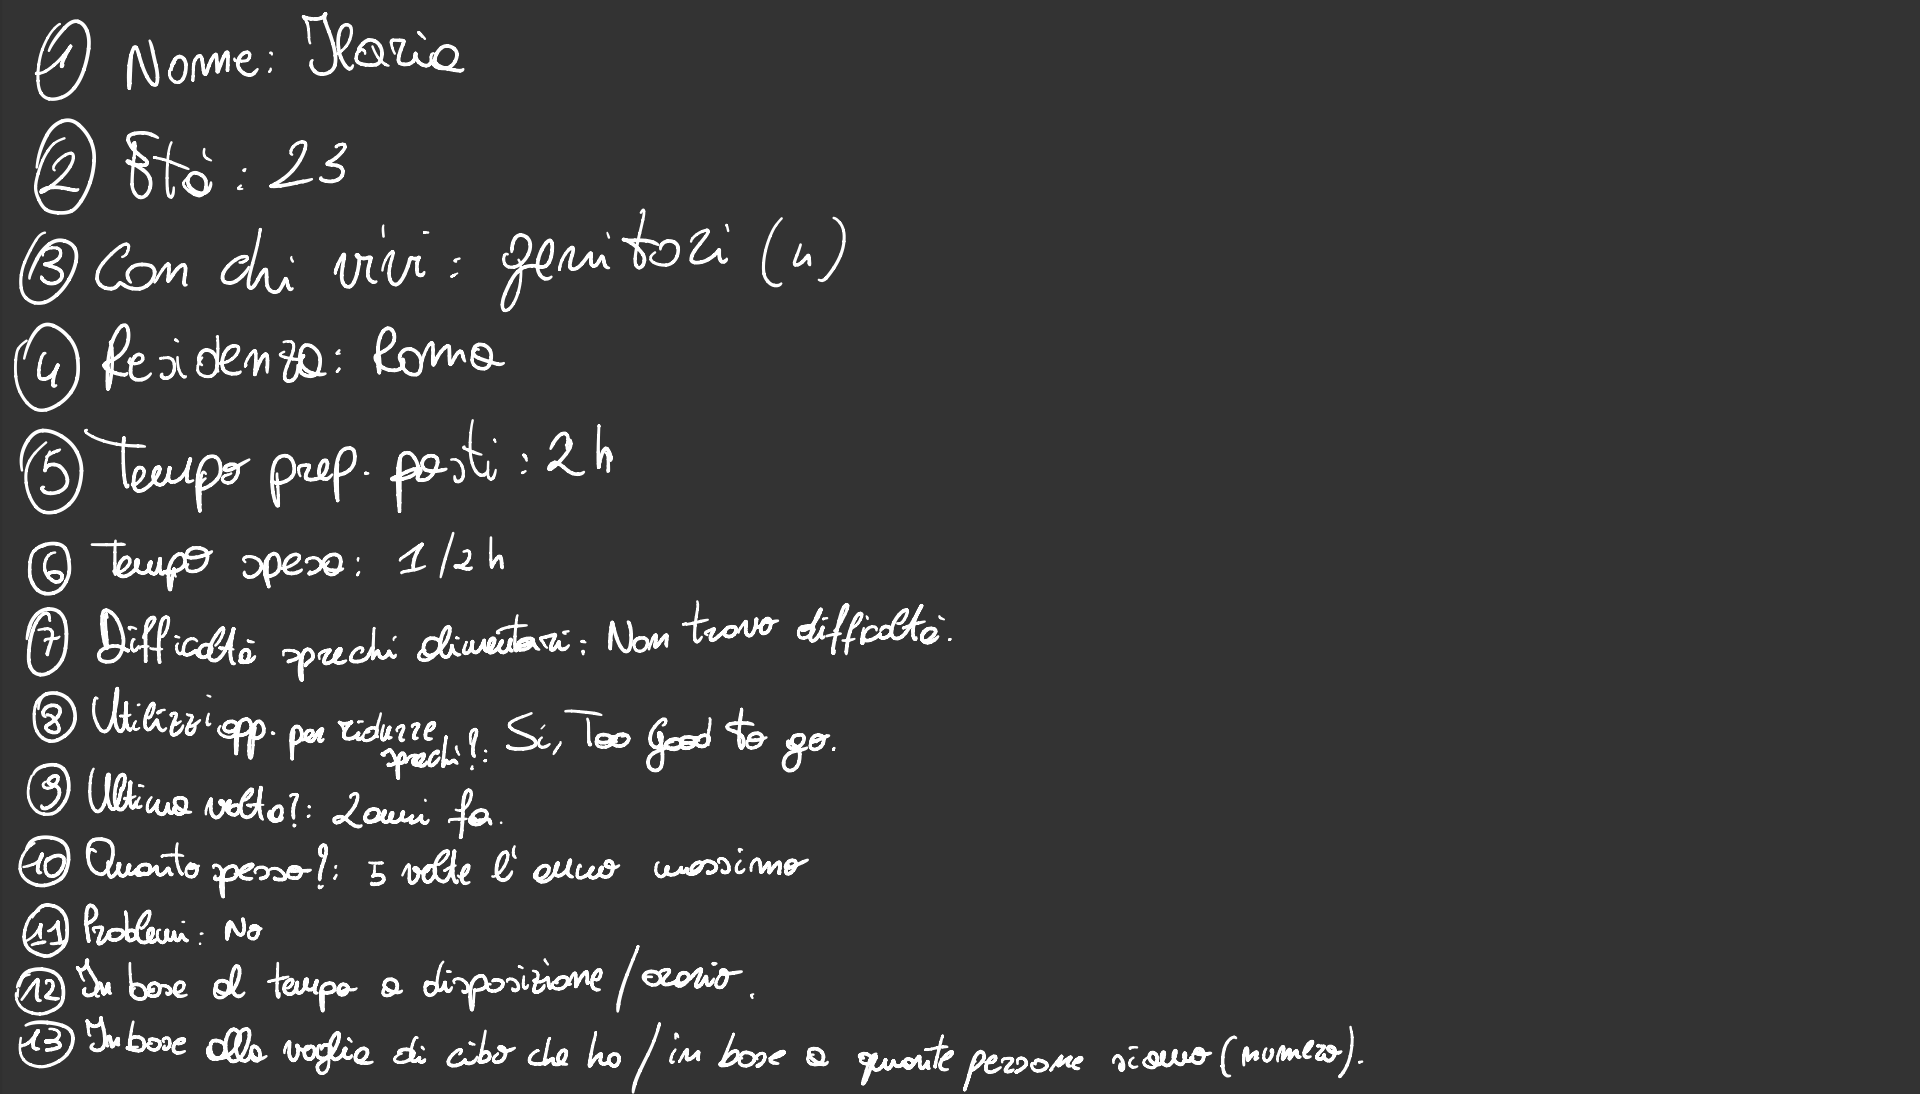
\includegraphics[width=\textwidth]{img/int5.png}
        \caption{Intervista 5}
    \end{subfigure}
    \hfill
    \begin{subfigure}{0.40\textwidth}
        \centering
        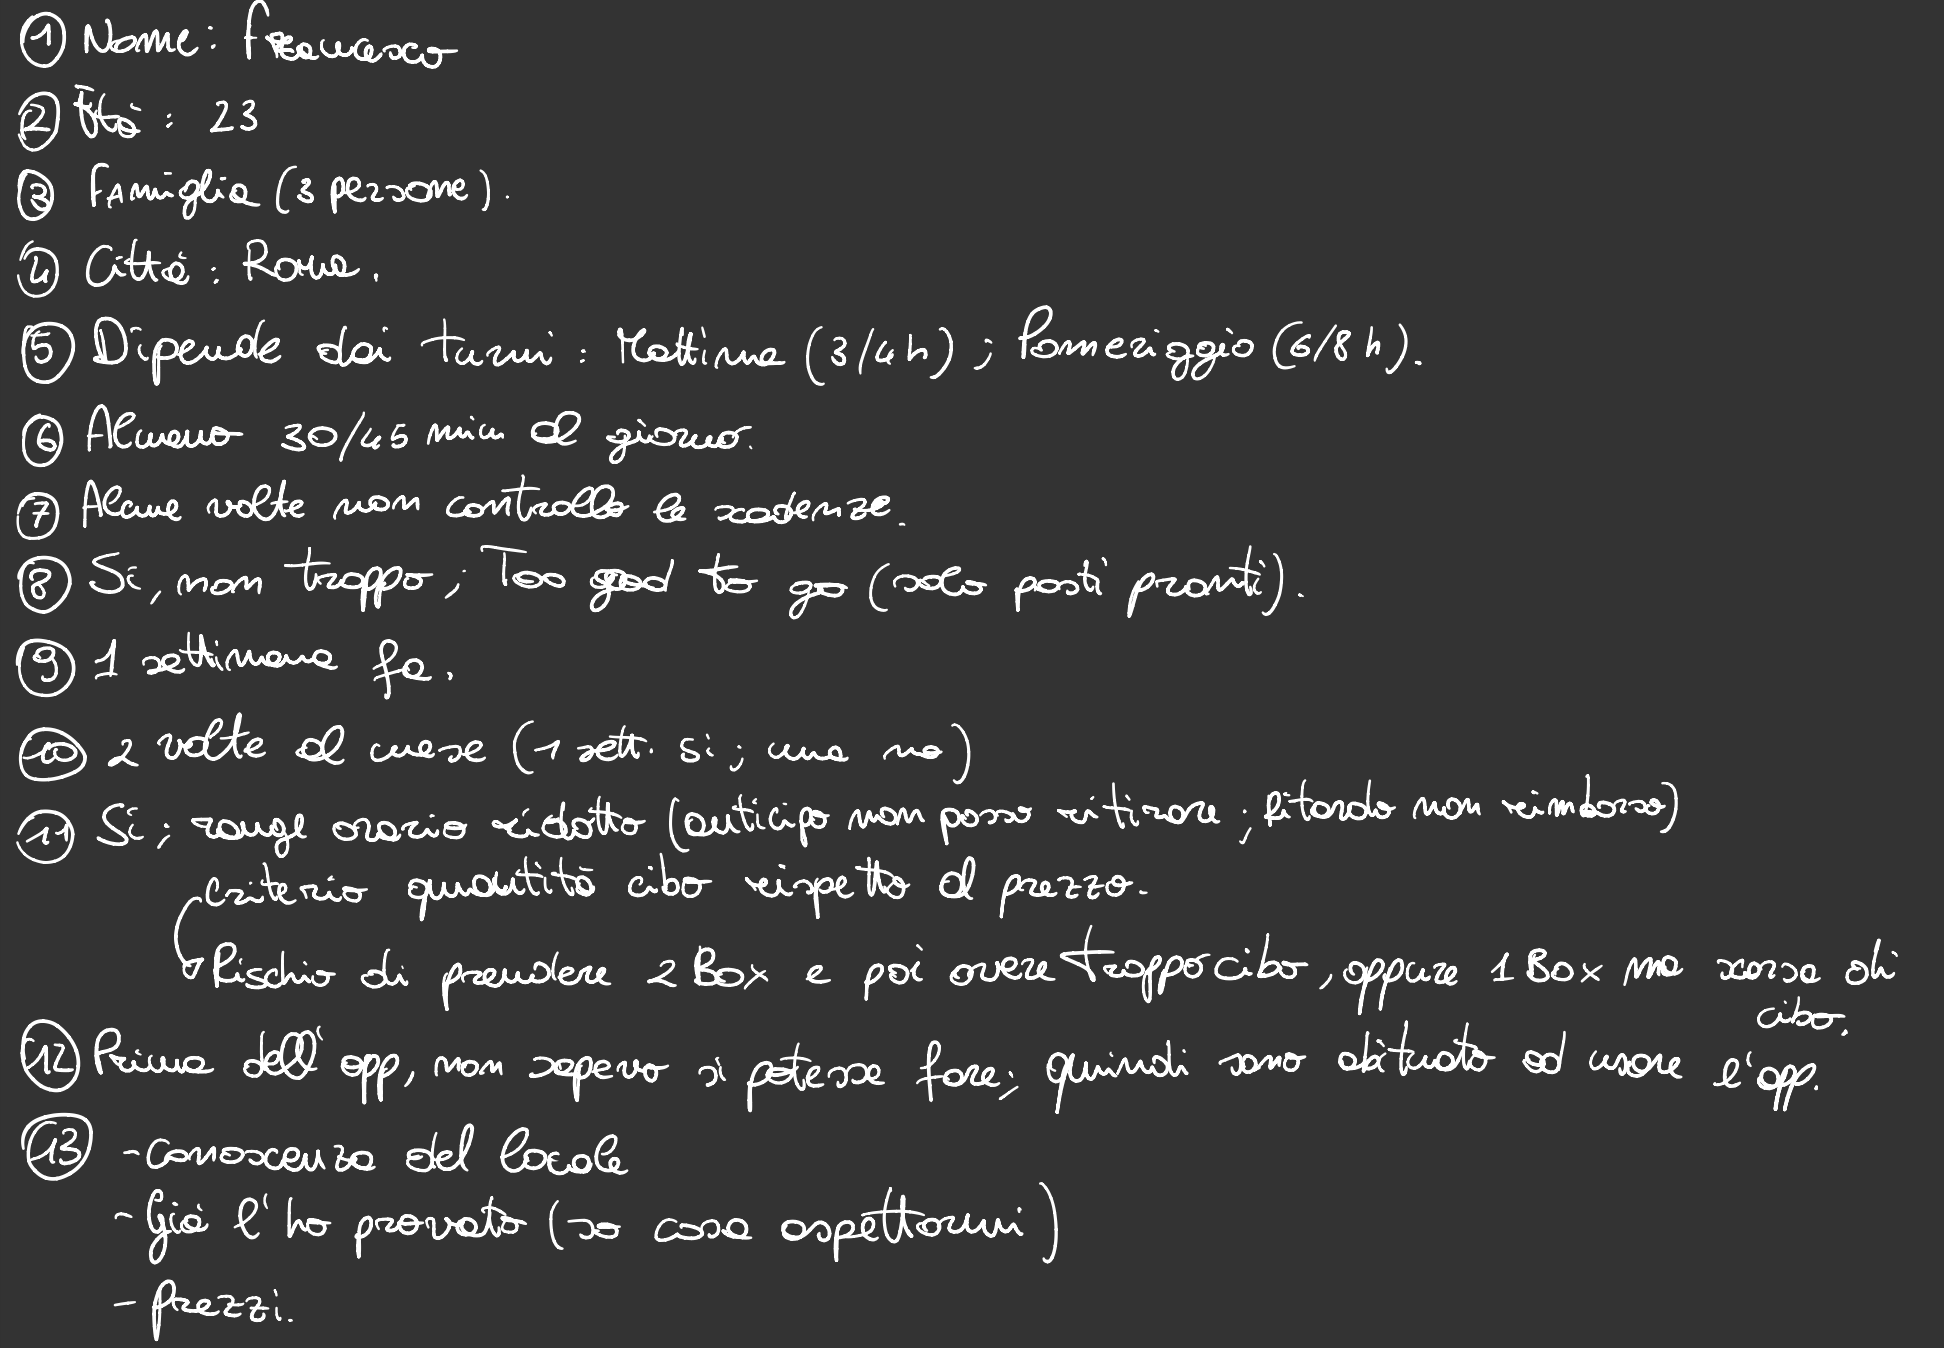
\includegraphics[width=\textwidth]{img/int6.png}
        \caption{Intervista 6}
    \end{subfigure}
\end{figure}

\end{document}